 
\section{An Overview of the Architecture}
\label{sec:implementation_intro}

In this chapter I am going to enter into the details of the implementation of
the platform. The platform consists of three main pieces:

\mylist
  \item The {\bf Storm} application. This application is responsible of all the
computations being made. It is the main piece of the platform and it will be
thoroughly explained in the sections \ref{sec:implementation_core},
\ref{sec:implementation_aqs} and \ref{sec:implementation_bsp}.
  \item The {\bf Cassandra} instance. This instance is shated among all the
other pieces and stores the state of the platform. We will enter in more detail
later on this chapter about what is the state of the platform.
  \item The {\bf API} layer. This is a very thin layer that is placed between
the Storm application and the end developer. The API is explained in section
\ref{sec:implementation_api}.
\mylistend

The architecture itself is a bit complicated, since we want to provide a
realtime API. Nonetheless, one can have a general idea of the architecture with
the following image:

\begin{center}
  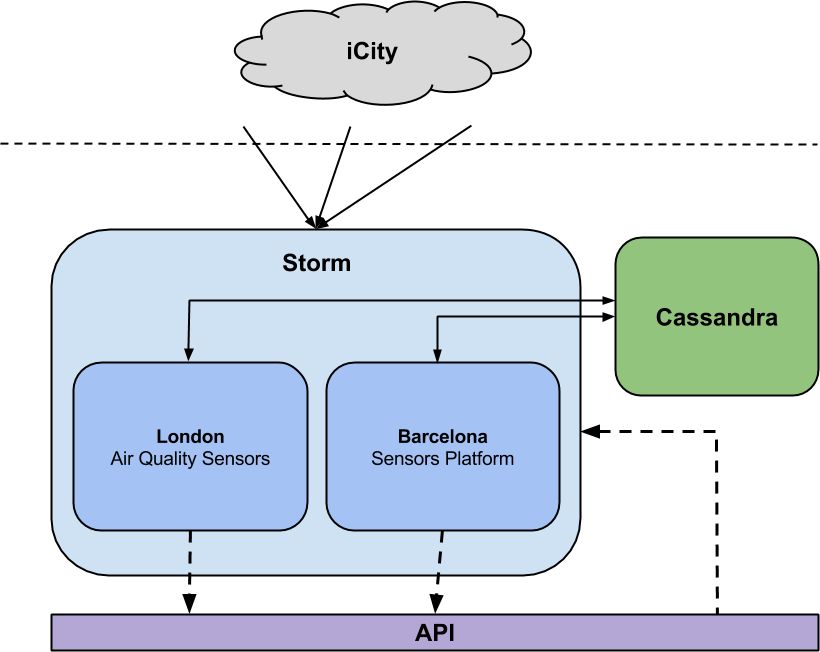
\includegraphics[scale=0.5]{implementation/images/platform.png}
\end{center}

\subsubsection*{iCity}

As you can see, the iCity platform is represented as a cloud. This is because
we do not really care about the internal infrastructure of the iCity platform.
The only thing we care about iCity, from a developer perspective, is that it
has an API that integrates all its resources.

Therefore, our point of view is: we receive data from a platform called iCity,
and we do not want to know what is going on inside this platform. Of course,
since this platform is totally independent to the source (iCity), we could
ideally add more ``clouds'' without too many problems. This change would
require a few and trivial changes in the code of the Storm application.

\subsubsection*{Cassandra}

Cassandra is a NoSQL Database Management System that works wonderfully in
clusters. For more information about Cassandra, you might want to read
section \ref{sec:cassandra}. The main point of Cassandra is that it is designed
to work on cluster and that it can be fully integrated in a Storm application.

Now, why would we want a Database Management System? The answer is that we need
to store the {\bf state} of the application. By state we mean some data that is
relevant to the whole application. An example of the data that we store in
Cassandra are devices. Each city has a set of devices, and these devices have a
set of properties. The iCity API expect the developer to request information by
pairs of deviceID-property. Therefore, we need to store the devices for each
city and the properties that we can request from them. In the future we could
add statistics about the execution of the application for debugging purposes.

The point is that Cassandra is an important piece of the puzzle but the data
stored will not grow too much since the state of the application does not
require a lot of data.

\subsubsection*{Storm and the API}

As you can see in the picture, there are dashed arrows between the Storm
application and the API. These arrows are drawn this way because they are TCP
sockets between Storm and the API.

A Storm application consists of a topology of spouts and bolts. The spouts
fetch the data continously. In our case this data comes from the iCity
platform. The output of the Storm application is given by the bolts in the end
of the topology. This output is given continously, because of the nature of the
Storm application. Therefore, we need sockets to pass the results from the
Storm application to the API layer.

But, how can the Storm application know the address and port of the sockets?
This information is given by the API. In short, when the API has a new request,
it creates a new TCP socket, and the address and port of this new socket will
be passed to the Storm application. You can see this in the picture represented
as the rightmost dashed arrow. You can think of this as subscriptions:

\mylist
  \item The API opens a new socket for each request and subscribes it in the
Storm application.
  \item The action of ``subscribe'' is done through a socket that the Storm
application is listening to.
  \item It is up to the API layer to keep the streaming model. This means that
the API can stream the data received from the socket to the end developer or it
can decide to close the connection after a certain period of time. This means
that this API is, by design, able to offer both ``traditional'' endpoints or
streaming endpoints. We will see more about this in section
\ref{sec:implementation_bsp}.
\mylistend
